\documentclass[slidestop,mathserif]{beamer}

\usetheme{Madrid}
\usecolortheme{seahorse}

\usepackage{geometry}
\usepackage{graphicx}
\usepackage{amssymb}
\usepackage{epstopdf}
\usepackage{amsmath}  	% this permits text in eqnarray among other benefits
\usepackage{color}          	% gives color options
\usepackage{url}		% produces hyperlinks
\usepackage[english]{babel}
\usepackage[latin1]{inputenc}
\usepackage{colortbl}	% allows for color usage in tables
\usepackage{multirow}	% allows for rows that span multiple rows in tables
\usepackage{xcolor}		% this package has a variety of color options
\usepackage{calc}
\usepackage{multicol}

\setbeamertemplate{navigation symbols}{}

%User defined colors: See colors section
\xdefinecolor{oiBlue}{rgb}{0.15, 0.35, 0.55}
\xdefinecolor{gray}{rgb}{0.5, 0.5, 0.5}
\xdefinecolor{darkGray}{rgb}{0.3, 0.3, 0.3}
\xdefinecolor{darkerGray}{rgb}{0.2, 0.2, 0.2}
\xdefinecolor{rubineRed}{rgb}{0.89,0,0.30}
\xdefinecolor{linkCol}{rgb}{0.11,0.49,0.95}	
\xdefinecolor{irishGreen}{rgb}{0,0.60,0}	
\xdefinecolor{darkturquoise}{rgb}{0.44, 0.58, 0.86}
\definecolor{lightGreen}{rgb}{0.533,0.765,0.42}

\setbeamercolor*{palette primary}{fg=white,bg= oiBlue!70}
\setbeamercolor*{palette secondary}{fg=black,bg= oiBlue!20!white}
\setbeamercolor*{palette tertiary}{fg=white,bg= oiBlue!80!black!90}
\setbeamercolor*{palette quaternary}{fg=white,bg= oiBlue}

\setbeamercolor{structure}{fg= oiBlue}
\setbeamercolor{frametitle}{bg= oiBlue!70}

\setbeamercolor{disc body}{bg=oiBlue!20!white!80,fg=oiBlue!80!black!90}
\setbeamercolor{disc title}{bg=oiBlue!40!white!60,fg=oiBlue!70!black!100}


\setbeamertemplate{blocks}[shadow=false]


\newcommand{\removepagenumbers}{% 
  \setbeamertemplate{footline}{
    %
    \begin{beamercolorbox}[colsep=1.5pt]{upper separation line foot}
    \end{beamercolorbox}
    \begin{beamercolorbox}[ht=2.5ex,dp=1.125ex,%
      leftskip=.3cm,rightskip=.3cm plus1fil]{author in head/foot}%
      \leavevmode{\usebeamerfont{author in head/foot}\insertshortauthor}%
%      \hfill%
%      {\usebeamerfont{author in head/foot}\usebeamercolor[fg]{institute in head/foot}\insertshortinstitute}%
    \end{beamercolorbox}%
    \begin{beamercolorbox}[ht=2.5ex,dp=1.125ex,%
      leftskip=.3cm,rightskip=.3cm plus1fil]{title in head/foot}%
      {\usebeamerfont{title in head/foot}\insertshorttitle}%
      \hfill%
      {\usebeamerfont{author in head/foot}\usebeamercolor[fg]{institute in head/foot}\insertshortinstitute}%
    \end{beamercolorbox}%
    \begin{beamercolorbox}[colsep=1.5pt]{lower separation line foot}
    \end{beamercolorbox}
    }
} 


\newcommand{\disc}[2]{
\begin{beamerboxesrounded}[shadow = true, lower = disc body, upper = disc title]{#1}
#2
\end{beamerboxesrounded}
}


\AtBeginSection[] 
{ 
  \addtocounter{framenumber}{-1} 
  % 
  {\removepagenumbers 
    \begin{frame}<beamer> 
    \tableofcontents[currentsection] 
  \end{frame} 
  } 
} 

\setbeamertemplate{navigation symbols}{}

\usepackage{minted}

\title[rgeos]{{\LARGE \texttt{rgeos}}\\ {\small spatial geometry predicates and topology operations in R}}
\author[Rundel, Bivand, Pebesma]{Colin Rundel (Duke University) \\ Roger Bivand (Norwegian School of Economics) \\ Edzer Pebesma (University of M\"unster)}
\date{June 14, 2012}
%\institute{Duke University}

\begin{document}

\begin{frame}[plain]
\titlepage
\end{frame}

%%%%%%%%%%%%%%%%%%%%%%%%%%%%%%%%%%%%
%%%%%%%%%%%%%%%%%%%%%%%%%%%%%%%%%%%%
\section{rgeos}
%%%%%%%%%%%%%%%%%%%%%%%%%%%%%%%%%%%%
%%%%%%%%%%%%%%%%%%%%%%%%%%%%%%%%%%%%

%%%%%%%%%%%%%%%%%%%%%%%%%%%%%%%%%%%%
%%%%%%%%%%%%%%%%%%%%%%%%%%%%%%%%%%%%
\subsection{Background}
%%%%%%%%%%%%%%%%%%%%%%%%%%%%%%%%%%%%
%%%%%%%%%%%%%%%%%%%%%%%%%%%%%%%%%%%%

\begin{frame}
\frametitle{Package Overview}

\only<1>{
What is GEOS?
\begin{itemize}
\item Implements all the OpenGIS Consortium's Simple Feature Access for SQL specification
\item C++ port of the Java Topology Suite
\item Available under the LGPL
\item Geometry engine behind open source project like PostGIS, SpatiaLite, QGIS, ...
\end{itemize}
}
\only<2>{
What is \texttt{rgeos}?
\begin{itemize}
\item Brings the functionality of GEOS to R
\item Developed in collaboration with Roger Bivand and Edzer Pebesma
\item Official GSoC project in Summer 2010
\item Implements the majority of the v1.6.2 C API (GEOS 3.2.2 and above)
\item Written to integrate with R spatial packages (\texttt{sp}, \texttt{maptools}, etc.)
\item Available on CRAN
\end{itemize}
}
\end{frame}

%%%%%%%%%%%%%%%%%%%%%%%%%%%%%%%%%%%%
%%%%%%%%%%%%%%%%%%%%%%%%%%%%%%%%%%%%
\subsection{Functionality}
%%%%%%%%%%%%%%%%%%%%%%%%%%%%%%%%%%%%
%%%%%%%%%%%%%%%%%%%%%%%%%%%%%%%%%%%%

\begin{frame}
\frametitle{OGC Simple Feature Access for SQL}

Common standard for the representation of Geospatial data
\begin{itemize}
\item Specifies common 2d geometric data types:
\begin{multicols}{2}
\begin{itemize}
\item Point / MultiPoint
\item LineString / MultiLineString
\item Polygon / MultiPolygon
\item LinearRing
\item GeometryCollection
\end{itemize}
\end{multicols}
\item Also specifies attributes, methods, and assertions for these geometries
\item Common exchange formats: Well-known text, Well-known binary
\item Standard - \urlwofont{http://www.opengeospatial.org/standards/sfs}
\end{itemize}

\end{frame}

%%%%%%%%%%%%%%%%%%%%%%%%%%%%%%%%%%%%

\begin{frame}
\frametitle{\texttt{sp} and SFS}
\texttt{sp} classes are very similar but differ in several important ways from SFS data types

\begin{itemize}
\item No native support for GeometryCollections or LinearRings (SpatialRings and SpatialCollections added in rgeos)
\item Translation / implementation ambiguities
\begin{itemize}
\item Should a SpatialPolygons object be a single MultiPolygon or a collection of polygons to iterate over?
\end{itemize}
\item Differences in Polygon implementation
\end{itemize}

\end{frame}

%%%%%%%%%%%%%%%%%%%%%%%%%%%%%%%%%%%%

\begin{frame}
\frametitle{Topology Operations}

\begin{beamerboxesrounded}{Boolean}
\begin{multicols}{3}
\begin{itemize}
\item gDifference
\item gIntersection
\item gSymdifference
\item gUnion
\end{itemize}
\end{multicols}
\end{beamerboxesrounded}
~\\
\begin{beamerboxesrounded}{Constructive}
\begin{multicols}{3}
\begin{itemize}
\item gBoundary
\item gBuffer
\item gCentroid
\item gConvexHull
\item gEnvelope
\item gLineMerge
\item gPointOnSurface
\item gPolygonize
\item gSimplify
\item gUnionCascaded / gUnionUnary
\end{itemize}
\end{multicols}
\end{beamerboxesrounded}
~\\
\begin{beamerboxesrounded}{Metric}
\begin{multicols}{3}
\begin{itemize}
\item gArea
\item gDistance
\item gLength
\end{itemize}
\end{multicols}
\end{beamerboxesrounded}


\end{frame}

%%%%%%%%%%%%%%%%%%%%%%%%%%%%%%%%%%%%

\begin{frame}
\frametitle{Topology - Boolean}

\begin{center}
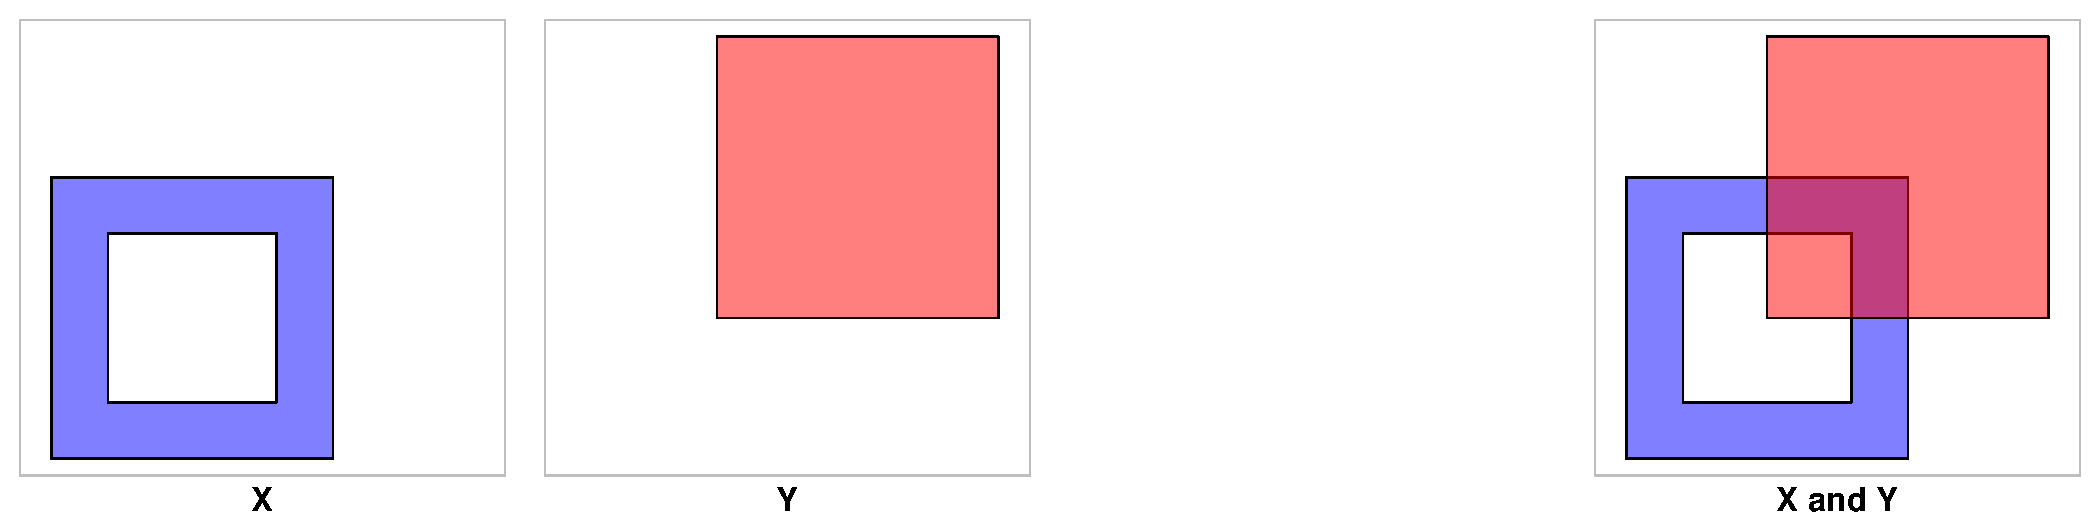
\includegraphics[width=\textwidth]{Figures/booleans1.pdf} \\
\pause
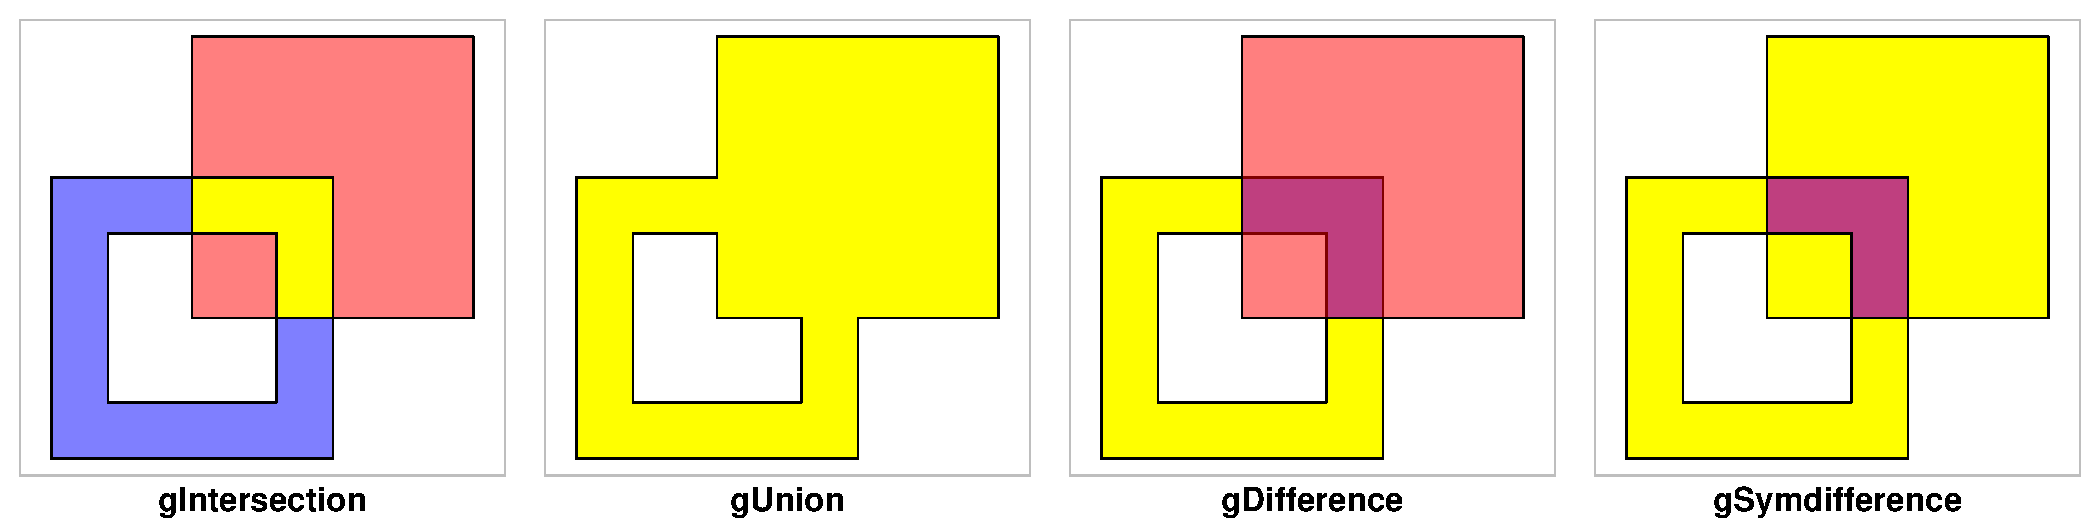
\includegraphics[width=\textwidth]{Figures/booleans2.pdf} \\
\end{center}

\end{frame}

%%%%%%%%%%%%%%%%%%%%%%%%%%%%%%%%%%%%

\begin{frame}
\frametitle{\texttt{rgeos} and \texttt{gpclib}}

The original impetus for \texttt{rgeos} was the need to replace Roger Peng's \texttt{gpclib} package which implemented these boolean operations for polygons.

\begin{itemize}
\item \texttt{gpclib} is a wrapper around Alan Murta's General Polygon Clipper library
\item The GPC library has a restrictive license (free only for non-commercial use)
\item The GPC library is limited to polygon clipping (boolean operations)
\item \texttt{gpclib} uses gpc.poly S4 classes
\end{itemize}
\vspace{3mm}
\texttt{rgeos} has functionality to transparently replace \texttt{gpclib} for purposes of backwards compatibility

\end{frame}

%%%%%%%%%%%%%%%%%%%%%%%%%%%%%%%%%%%%

\begin{frame}[fragile]
\frametitle{Topology - Constructive}
\begin{example}
{\scriptsize
\begin{minted}{r}
library(maptools)
nc = readShapePoly(
        system.file("shapes/sids.shp", package="maptools")[1], 
        proj4string=CRS("+proj=longlat +datum=NAD27")
     )
pts = coordinates(nc)
ID = cut(pts[,1], quantile(pts[,1]), include.lowest=TRUE)
nc_regions = gUnionCascaded(nc, ID)
\end{minted}
% 
% pdf("Figures/nc.pdf",height=3.5); par(mar=c(1,1,1,1)); plot(nc);dev.off()
% pdf("Figures/nc_regions.pdf",height=3.5); par(mar=c(1,1,1,1)); plot(nc_regions);dev.off()
%
}
\end{example}

\begin{center}
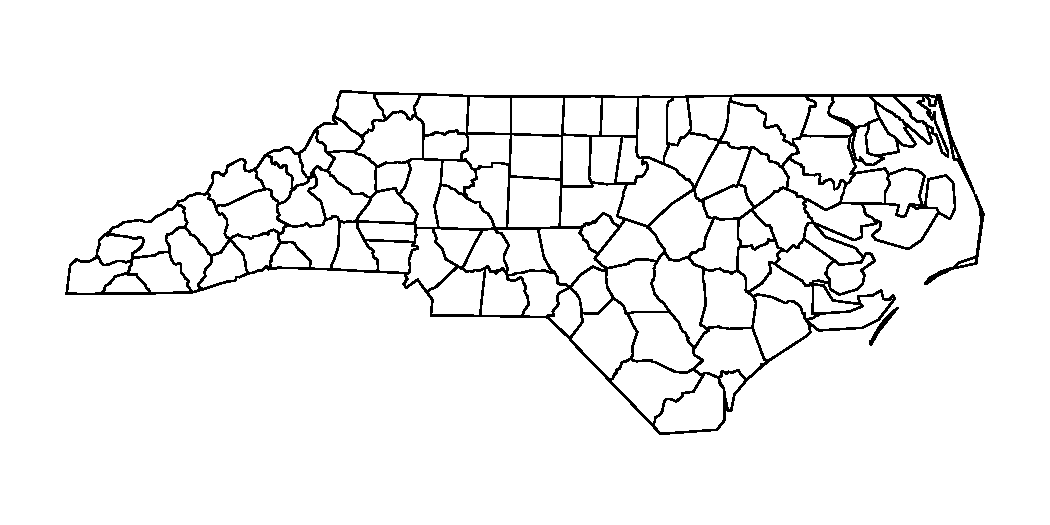
\includegraphics[width=2in]{Figures/nc.pdf} \pause
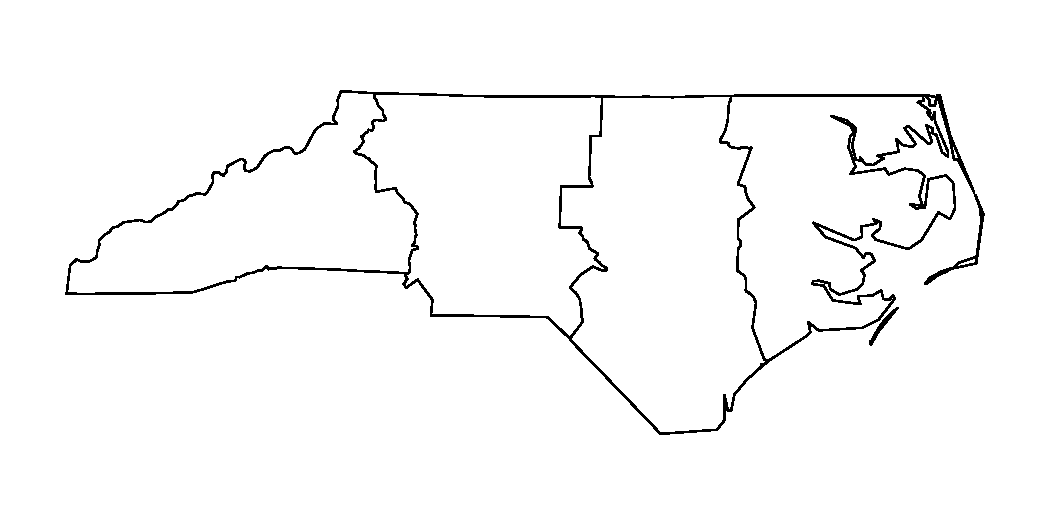
\includegraphics[width=2in]{Figures/nc_regions.pdf}
\end{center}

\end{frame}

%%%%%%%%%%%%%%%%%%%%%%%%%%%%%%%%%%%%

\begin{frame}
\frametitle{Spatial Predicates}

\begin{beamerboxesrounded}{Unary}
\begin{multicols}{3}
\begin{itemize}
    \item gIsEmpty
    \item gIsRing
    \item gIsSimple
    \item gIsValid
\end{itemize}
\end{multicols}
\end{beamerboxesrounded}
~\\
\begin{beamerboxesrounded}{Binary}
\begin{multicols}{3}
\begin{itemize}
    \item gContains
    \item gContainsProperly
    \item gCovers
    \item gCoveredBy
    \item gCrosses
    \item gDisjoint
    \item gEquals
    \item gEqualsExact
    \item gOverlaps
    \item gRelate
    \item gTouches
    \item gWithin
    \item gWithinDistance
\end{itemize}
\end{multicols}
\end{beamerboxesrounded}

\vfill

{\scriptsize Package Documentation and JTS Technical Specifications cover the specifics of these functions (\urlwofont{http://bit.ly/L1uifo})}

\end{frame}

\begin{frame}
\frametitle{gRelate and DE-9IM}

Binary predicates are based on the Dimensionally Extended 9-Intersection Model

\begin{itemize}
\item Reports the dimensionality of the intersection of the interiors, boundaries, and exteriors
\item Possible values: 0, 1, 2, F, T, *
\end{itemize}

\only<1>{
\begin{columns}[c]
\column{0.1\textwidth}
\column{0.6\textwidth}
\begin{center}
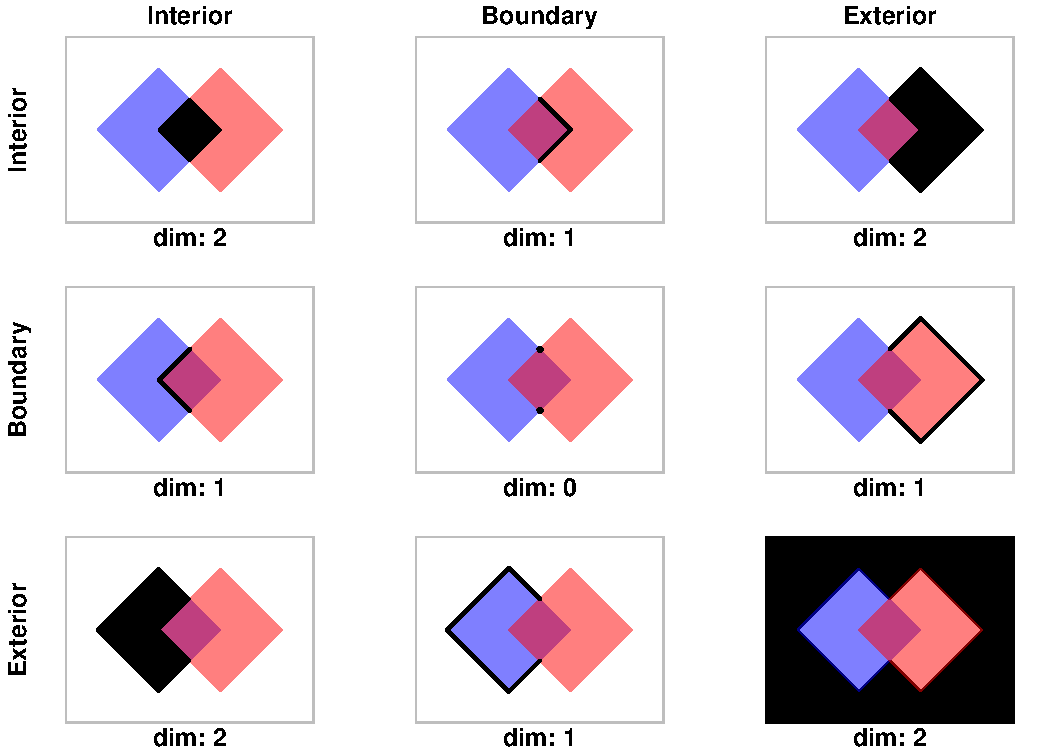
\includegraphics[width=0.9\textwidth]{Figures/de9im.pdf}
\end{center}
\column{0.3\textwidth}
{\large $\Rightarrow$ ``212101212''}
\end{columns}
}

\only<2>{
\begin{center}
\begin{tabular}{l|l|l}
DE-9IM Pattern   & Function  & f(x,y) \\
\hline
FF*FF****        & gDisjoint & false  \\
FT*******        & gTouches  & false  \\
T*T***T**        & gCrosses  & true   \\
TF*F*****        & gWithin   & false  \\
T*T***T**        & gOverlaps & true   \\   
\end{tabular}
\end{center}
\vfill

{\footnotesize For a more details - \urlwofont{http://bit.ly/Kxm6iz} or \urlwofont{http://bit.ly/L1uifo}}
}

\end{frame}

%%%%%%%%%%%%%%%%%%%%%%%%%%%%%%%%%%%%

\begin{frame}
\frametitle{Spatial Predicates and Prepared Geometries}

Common usage pattern with spatial predicates will involve a single geometry being compared to a series of test geometries.
\begin{itemize}
\item Initial Geometry is reused for each subsequent predicate
\item Many of the underlying calculations / data structures can be cached
\item In some cases evaluation steps can be skipped
\item Potentially huge performance gains for minimal overhead (on by default when possible)
\item This is an area of recent development activity for GEOS:
\begin{itemize}
\item CAPI v1.6.2 (GEOS v3.2.2) supports: Contains, ContainsProperly, Covers, Intersects
\item CAPI v1.7.0 (GEOS v3.3+) added support for: CoveredBy, Crosses, Disjoint, Overlaps, Touches, Within
\end{itemize}
\end{itemize}

\end{frame}

%%%%%%%%%%%%%%%%%%%%%%%%%%%%%%%%%%%%

\begin{frame}[fragile]
\frametitle{Prepared Geometry Performance}

\begin{example}
{\footnotesize
\begin{minted}{r}
library(maptools)

data(wrld_simpl)
US = wrld_simpl[wrld_simpl@data$NAME == "United States",]

gt = GridTopology(c(-180,-90),c(0.5,0.5),c(720,360))
grid = SpatialGrid(gt)
sp = as(grid, "SpatialPoints")
proj4string(sp) = proj4string(US)

system.time(gIntersects(US,sp,byid=TRUE,prepared=TRUE))
system.time(gIntersects(US,sp,byid=TRUE,prepared=FALSE))
\end{minted}
}
\end{example}

~\\ \pause

\begin{columns}
\column{0.05\textwidth}
\column{0.425\textwidth}
\begin{beamerboxesrounded}{prepared=TRUE}
\begin{minted}{r}
   user  system elapsed 
  0.220   0.016   0.285
\end{minted}
\end{beamerboxesrounded}

\column{0.05\textwidth}
\column{0.425\textwidth}
\begin{beamerboxesrounded}{prepared=FALSE}
\begin{minted}{r}
   user  system elapsed 
244.851   0.004 244.895
\end{minted}
\end{beamerboxesrounded}
\column{0.05\textwidth}
\end{columns}
\end{frame}

%%%%%%%%%%%%%%%%%%%%%%%%%%%%%%%%%%%%
%%%%%%%%%%%%%%%%%%%%%%%%%%%%%%%%%%%%
\subsection{Conclusion}
%%%%%%%%%%%%%%%%%%%%%%%%%%%%%%%%%%%%
%%%%%%%%%%%%%%%%%%%%%%%%%%%%%%%%%%%%

\begin{frame}
\frametitle{Future Work}

\begin{itemize}
\item Complete update to GEOS C API 1.7.0 while preserving backwards compatibility \\
~\\
\item Refine usability of STRtree spatial indexes \\
~\\
\item Add support for WKB  \\
~\\
\item Clean up documentation / Package vignette \\
~\\
\item Better handling of Spatial*DataFrames
\end{itemize}

\end{frame}

%%%%%%%%%%%%%%%%%%%%%%%%%%%%%%%%%%%%

\begin{frame}
\frametitle{Questions, Comments, Bugs?}
\vfill
{\Large
\renewcommand*\arraystretch{1.5}
\begin{tabular}{lll}
email        & : & rundel@gmail.com \\
mailing list & : & R-sig-Geo \\
r-forge      & : & {\normalsize \urlwofont{http://r-forge.r-project.org/projects/rgeos}} \\
github       & : & {\normalsize \urlwofont{http://github.com/rundel/rgeos}} \\
presentation & : & {\normalsize \urlwofont{http://github.com/rundel/UseR2012}} \\
\end{tabular}
}
\vfill
\end{frame}

\end{document}
